\documentclass[border=2mm]{standalone}
\setlength{\textwidth}{12.2cm}
\setlength{\textheight}{19.3cm}
\usepackage{pgf-pie}

\renewcommand{\scalefont}[1]{\large}

\begin{document}
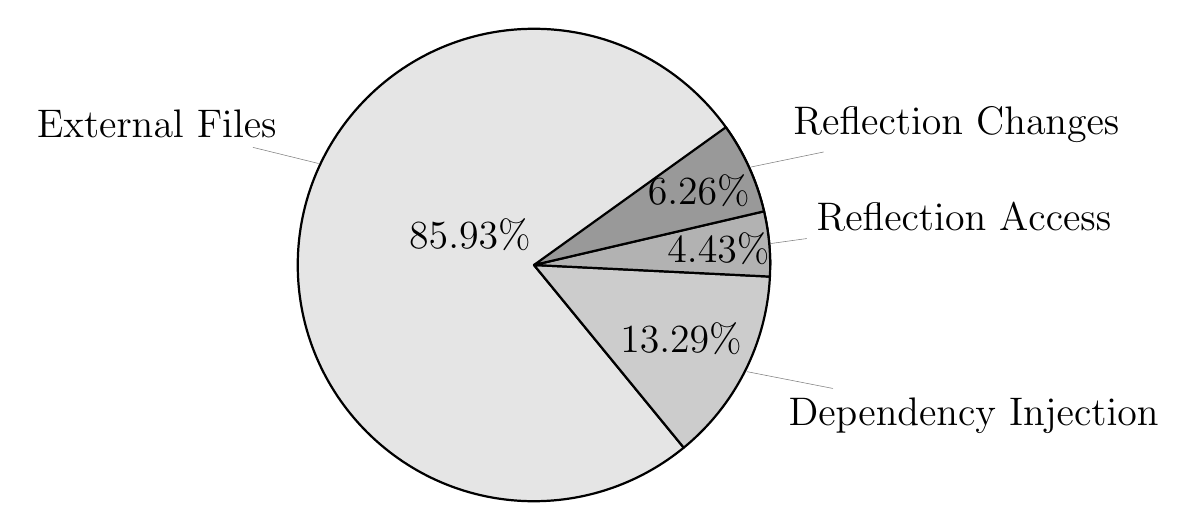
\begin{tikzpicture}
    % DATA:
    % 10000 Commits, 1151 detected commits with one source of unsafety, counted multiple times for
    % multiple unsafeties. Percentages rounded to two decimal places
    % 989 External Files -> 989 / 1151 * 100 -> 85.93
    % 153 Dependency Injection -> 153 / 1151 * 100 -> 13.29
    % 51 Reflection Access -> 51 / 1151 * 100 -> 4.43
    % 72 Reflection Changes -> 72 / 1151 * 100 -> 6.26
    \pie[
        /tikz/nodes={text=black, font=\Large},
        color={black!10, black!20, black!30, black!40},
        text=pin
    ]{
        85.93/External Files,
        13.29/Dependency Injection,
        4.43/Reflection Access,
        6.26/Reflection Changes
    }
\end{tikzpicture}
\end{document}
